%==============================================================================
\section{Fundamentação Teórica e Tecnológica}\label{fundamentacaoTeorica}
%==============================================================================

\subsection{Modelagem de processos}
A modelagem de um processo de software é realizada para possibilitar o entendimento e a padronização do processo aplicado durante o desenvolvimento de um software. Podemos destacar alguns objetivos para modelar processos de softwares \cite{genvigir2003modelagem}, como:

\begin{itemize}
	\item Possibilitar a comunicação e o entendimento efetivo do processo;
	\item Facilitar a reutilização do processo (padronização);
	\item Apoiar a evolução do processo;
	\item Facilitar o gerenciamento do processo.
\end{itemize}

Vários fatores levam para padronização dos processos, alguns dos principais são permitir treinamento, gerenciamento, revisões,
ferramentas de suporte, utilizar processos padronizados, contribuir para a melhoria dos processos na organização com as experiências de projeto e fornecer uma base estrutural para medição do processo \cite{genvigir2003modelagem}.


A classificação dos elementos dentro de um processo de software pode ser classificado como elementos e relacionamentos. Um modelo de processo concreto consiste de instâncias desses tipos de relacionamentos e elementos. O processo consiste em atividades de cooperação concorrentes abrangendo atividades de manutenção, desenvolvimento, segurança, qualidade e gerenciamento de projeto. Os elementos e os relacionamentos permitem uma modelagem rústica de um processo de software. Sendo assim, uma linguagem de modelagem de processo de software deve fornecer recursos de linguagem para modelar esses elementos básicos e avançados bem como seus inter-relacionamentos. As variantes podem ser classificada de acordo com características. Como não é possível abranger todas as características dentro de uma linguagem de especificação, deve se tomar a decisão do que está relacionado a fase do meta-processo e quem está lidando com o modelo do processo na construção do modelo da linguagem \cite{genvigir2003modelagem}.


\subsection{Software Process Engineering Metamodel -- SPEM}


O SPEM é o metamodelo proposto pela da OMG\footnote{Google Scholar \url{http://www.omg.org/}} para a descrição de um processo concreto de desenvolvimento de software ou uma família de processos de desenvolvimento de software. O SPEM surgiu com o objetivo de unificar diferentes metodologias propostas para a modelagem de processos. Ele utiliza a orientação a objeto para modelar uma família relacionada de processos de software e usa a UML como notação.

Na Figura \ref{fig:niveisSpem} exibe as quatro arquiteturas de modelagem definidas pela OMG. SPEM se encontra no nível M2 da arquitetura e é definido usando um subconjunto da UML, semelhante como a UML realiza com o MOF, parte da UML utiliza as facilidades implementadas e apoiadas pelo MOF \cite{genvigir2003modelagem}.  

\begin{figure}[!htb]
	\caption{Gráfico do ano das publicações}\label{fig:niveisSpem}
	\begin{center}
		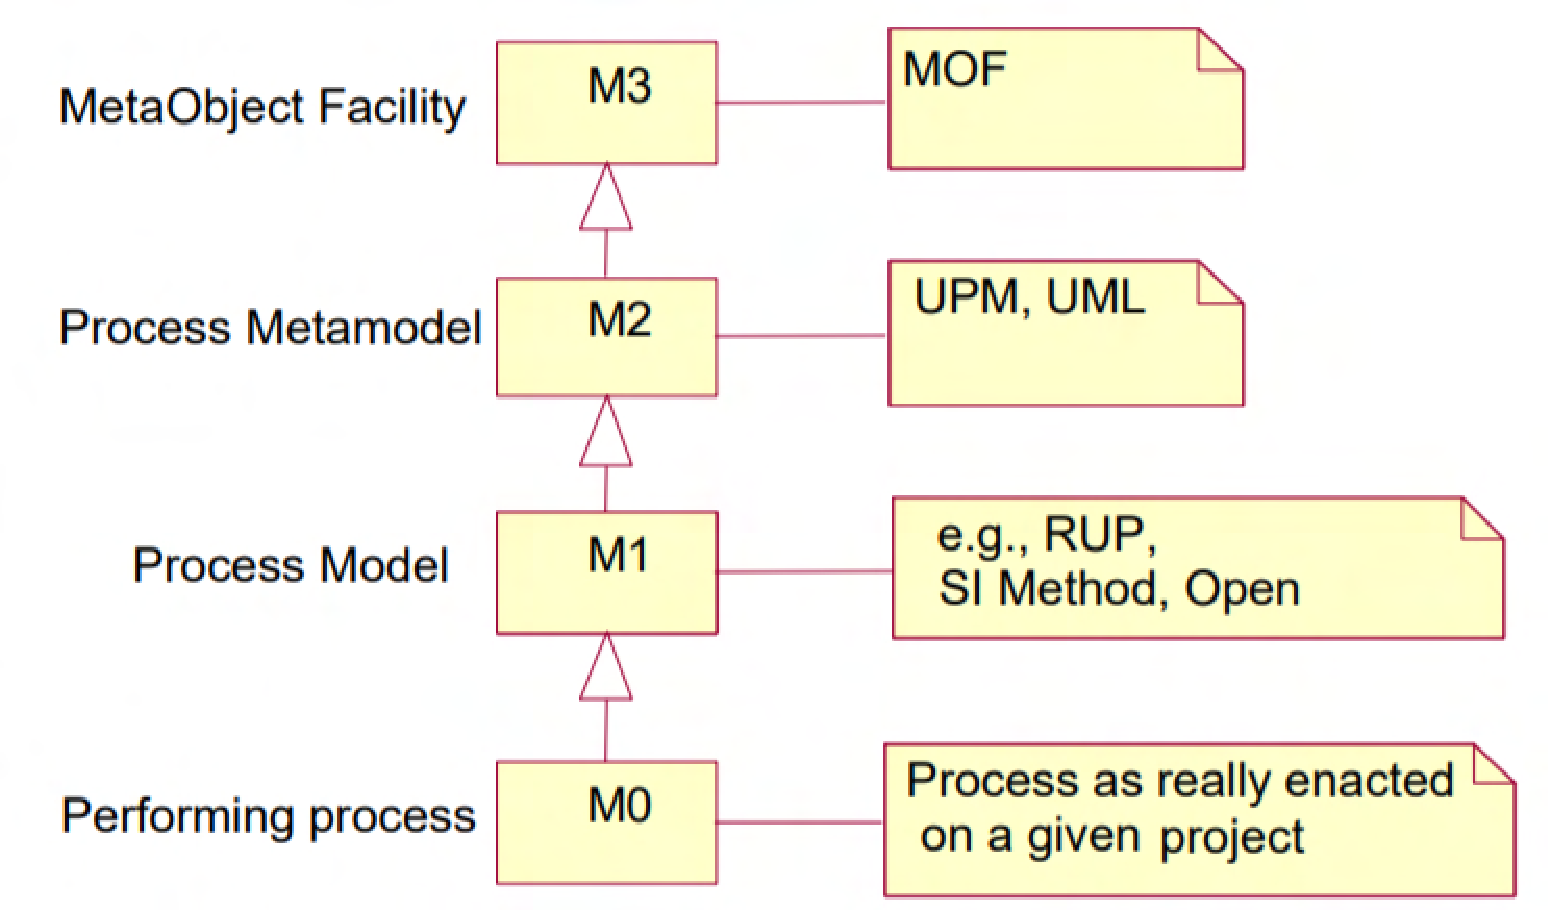
\includegraphics[scale=0.5]{img/spemNiveis}
	\end{center}
	%\legend{}
\end{figure}

Segundo a proposta do SPEM quando um processo é executado, aplicado no mundo real ele está no nível de M0. Um processo definido está no nível M1, como por exemplo o Processo Unificado Rational -- RUP. O SPEM pode ser usado para definir todos os tipos de processos, incluindo os focados no uso específico da UML. A UML é definida por um metamodelo, que é definido como uma instância do metamodelo MOF, localizado em M3. Como ja relatado apenas um subconjunto da notação gráfica da UML é usado para descrever este metamodelo. O metamodel SPEM foi elaborado similarmente, e é formalmente definido como uma extensão de um subconjunto da UML chamado SPEM\_Foundation \cite{genvigir2003modelagem}. 
